%%% title presen240828
\documentclass[landscape,10pt]{jarticle}
\usepackage{pict2e}
\usepackage{ketpic2e,ketlayer2e}
\special{papersize=\the\paperwidth,\the\paperheight}
\usepackage{ketslide}
\usepackage{amsmath,amssymb}
\usepackage{bm,enumerate}
\usepackage[dvipdfmx]{graphicx}
\usepackage{color}
\usepackage[dvipdfmx,colorlinks=true,linkcolor=blue,filecolor=blue]{hyperref}
\usepackage{emath,emathE,emathMw}

\def\deg#1{#1^{\circ}}
\newcommand{\monthday}{}

\definecolor{slidecolora}{cmyk}{0.98,0.13,0,0.43}
\definecolor{slidecolorb}{cmyk}{0.2,0,0,0}
\definecolor{slidecolorc}{cmyk}{0.2,0,0,0}
\definecolor{slidecolord}{cmyk}{0.2,0,0,0}
\definecolor{slidecolore}{cmyk}{0,0,0,0.5}
\definecolor{slidecolorf}{cmyk}{0,0,0,0.5}
\definecolor{slidecolori}{cmyk}{0.98,0.13,0,0.43}
\def\setthin#1{\def\thin{#1}}
\setthin{0}
\newcounter{pagectr}
\setcounter{pagectr}{1}
\newcommand{\slidepage}[1][\monthday-]{%
\setcounter{ketpicctra}{18}%

\begin{layer}{118}{0}
\putnotew{130}{-\theketpicctra.05}{\small#1\thepage/\pageref{pageend}}
\end{layer}

}

\setmargin{25}{145}{15}{100}

\ketslideinit

\pagestyle{empty}

\begin{document}

\begin{layer}{120}{0}
\putnotese{0}{0}{{\Large\bf
\color[cmyk]{1,1,0,0}

\begin{layer}{120}{0}
{\Huge \putnotes{60}{20}{インストール状況}}
\putnotes{60}{50}{高遠節夫}
\end{layer}

}
}
\end{layer}

\def\mainslidetitley{22}
\def\ketcletter{slidecolora}
\def\ketcbox{slidecolorb}
\def\ketdbox{slidecolorc}
\def\ketcframe{slidecolord}
\def\ketcshadow{slidecolore}
\def\ketdshadow{slidecolorf}
\def\slidetitlex{6}
\def\slidetitlesize{1.3}
\def\mketcletter{slidecolori}
\def\mketcbox{yellow}
\def\mketdbox{yellow}
\def\mketcframe{yellow}
\def\mslidetitlex{62}
\def\mslidetitlesize{2}

\color{black}
\Large\bf\boldmath
\addtocounter{page}{-1}

\renewcommand{\eda}[2][\theedactr]{%
\Ltab{\theedawidth mm}{[#1]\ #2}%
\addtocounter{edactr}{1}%
}
\def\dint{\displaystyle\int}
\def\bs#1{\textbackslash #1}
\renewcommand{\slidepage}[1][s]{%
\setcounter{ketpicctra}{18}%
\if#1m \setcounter{ketpicctra}{1}\fi
\hypersetup{linkcolor=black}%
\begin{layer}{118}{0}
\putnotee{125}{-\theketpicctra.05}{\small\monthday\thepage/\pageref{pageend}}
\end{layer}\hypersetup{linkcolor=blue}
}
%%%%%%%%%%%%

%%%%%%%%%%%%%%%%%%%%

\mainslide{KeTHistory}


\slidepage[m]
%%%%%%%%%%%%%

%%%%%%%%%%%%%%%%%%%%

\newslide{\ketpic}

\vspace*{18mm}

\slidepage
\textinit

\begin{layer}{120}{0}
\addtext{8}{}{2006}
\end{layer}

%%%%%%%%%%%%%

%%%%%%%%%%%%%%%%%%%%


\sameslide

\vspace*{18mm}

\slidepage
\textinit

\begin{layer}{120}{0}
\addtext{8}{}{2006}
\addtext{12}{\ten}{Mapleの関数データからTpicコードを生成}
\end{layer}


\sameslide

\vspace*{18mm}

\slidepage
\textinit

\begin{layer}{120}{0}
\addtext{8}{}{2006}
\addtext{12}{\ten}{Mapleの関数データからTpicコードを生成}
\addtext{12}{\ten}{Kisarazu Educational Tpic}
\end{layer}


\sameslide

\vspace*{18mm}

\slidepage
\textinit

\begin{layer}{120}{0}
\addtext{8}{}{2006}
\addtext{12}{\ten}{Mapleの関数データからTpicコードを生成}
\addtext{12}{\ten}{Kisarazu Educational Tpic}
\addtext{12}{\ten}{Mathematica, Scilab, Rバージョン}
\end{layer}


\sameslide

\vspace*{18mm}

\slidepage
\textinit

\begin{layer}{120}{0}
\addtext{8}{}{2006}
\addtext{12}{\ten}{Mapleの関数データからTpicコードを生成}
\addtext{12}{\ten}{Kisarazu Educational Tpic}
\addtext{12}{\ten}{Mathematica, Scilab, Rバージョン}
\addtext{12}{\ten}{ライブラリの行数は約15000}
\end{layer}


\sameslide

\vspace*{18mm}

\slidepage
\textinit

\begin{layer}{120}{0}
\addtext{8}{}{2006}
\addtext{12}{\ten}{Mapleの関数データからTpicコードを生成}
\addtext{12}{\ten}{Kisarazu Educational Tpic}
\addtext{12}{\ten}{Mathematica, Scilab, Rバージョン}
\addtext{12}{\ten}{ライブラリの行数は約15000}
\addtext{12}{\ten}{\TeX のマクロライブラリも作成}
\end{layer}


\newslide{\ketcindy}

\vspace*{18mm}

\slidepage
\textinit

\begin{layer}{120}{0}
\addtext{8}{}{2014}
\end{layer}

%%%%%%%%%%%%%

%%%%%%%%%%%%%%%%%%%%


\sameslide

\vspace*{18mm}

\slidepage
\textinit

\begin{layer}{120}{0}
\addtext{8}{}{2014}
\addtext{12}{\ten}{CinderellaでRの\ketpic コードを生成}
\end{layer}


\sameslide

\vspace*{18mm}

\slidepage
\textinit

\begin{layer}{120}{0}
\addtext{8}{}{2014}
\addtext{12}{\ten}{CinderellaでRの\ketpic コードを生成}
\addtext{12}{\ten}{CinderellaのJavaで一連の作業を実行}
\addtext{20}{}{Rのコード作成$\Rightarrow$R$\Rightarrow$TeX$\Rightarrow$PDFビューア}
\end{layer}


\sameslide

\vspace*{18mm}

\slidepage
\textinit

\begin{layer}{120}{0}
\addtext{8}{}{2014}
\addtext{12}{\ten}{CinderellaでRの\ketpic コードを生成}
\addtext{12}{\ten}{CinderellaのJavaで一連の作業を実行}
\addtext{20}{}{Rのコード作成$\Rightarrow$R$\Rightarrow$TeX$\Rightarrow$PDFビューア}
\addtext{12}{\ten}{インタラクティブに図が作成できる}
\end{layer}


\sameslide

\vspace*{18mm}

\slidepage
\textinit

\begin{layer}{120}{0}
\addtext{8}{}{2014}
\addtext{12}{\ten}{CinderellaでRの\ketpic コードを生成}
\addtext{12}{\ten}{CinderellaのJavaで一連の作業を実行}
\addtext{20}{}{Rのコード作成$\Rightarrow$R$\Rightarrow$TeX$\Rightarrow$PDFビューア}
\addtext{12}{\ten}{インタラクティブに図が作成できる}
\addtext{12}{\ten}{曲面描画ではGCCによる高速化}
\end{layer}


\sameslide

\vspace*{18mm}

\slidepage
\textinit

\begin{layer}{120}{0}
\addtext{8}{}{2014}
\addtext{12}{\ten}{CinderellaでRの\ketpic コードを生成}
\addtext{12}{\ten}{CinderellaのJavaで一連の作業を実行}
\addtext{20}{}{Rのコード作成$\Rightarrow$R$\Rightarrow$TeX$\Rightarrow$PDFビューア}
\addtext{12}{\ten}{インタラクティブに図が作成できる}
\addtext{12}{\ten}{曲面描画ではGCCによる高速化}
\addtext{12}{\ten}{pict2e,Tikzコードもサポートした}
\end{layer}


\sameslide

\vspace*{18mm}

\slidepage
\textinit

\begin{layer}{120}{0}
\addtext{8}{}{2014}
\addtext{12}{\ten}{CinderellaでRの\ketpic コードを生成}
\addtext{12}{\ten}{CinderellaのJavaで一連の作業を実行}
\addtext{20}{}{Rのコード作成$\Rightarrow$R$\Rightarrow$TeX$\Rightarrow$PDFビューア}
\addtext{12}{\ten}{インタラクティブに図が作成できる}
\addtext{12}{\ten}{曲面描画ではGCCによる高速化}
\addtext{12}{\ten}{pict2e,Tikzコードもサポートした}
\addtext{12}{\ten}{ライブラリの総行数は約30000}
\end{layer}


\newslide{\ketcindy JS}

\vspace*{18mm}

\slidepage
\textinit

\begin{layer}{120}{0}
\addtext{8}{}{2016}
\end{layer}

%%%%%%%%%%%%%

%%%%%%%%%%%%%%%%%%%%


\sameslide

\vspace*{18mm}

\slidepage
\textinit

\begin{layer}{120}{0}
\addtext{8}{}{2016}
\addtext{12}{\ten}{CindyJSでHTMLをエクスポート}
\end{layer}


\sameslide

\vspace*{18mm}

\slidepage
\textinit

\begin{layer}{120}{0}
\addtext{8}{}{2016}
\addtext{12}{\ten}{CindyJSでHTMLをエクスポート}
\addtext{12}{\ten}{使用されている\ketcindy の関数を再帰的に追加}
\end{layer}


\sameslide

\vspace*{18mm}

\slidepage
\textinit

\begin{layer}{120}{0}
\addtext{8}{}{2016}
\addtext{12}{\ten}{CindyJSでHTMLをエクスポート}
\addtext{12}{\ten}{使用されている\ketcindy の関数を再帰的に追加}
\addtext[8]{12}{\ten}{教材HTMLを簡単に作成できる}
\end{layer}


\sameslide

\vspace*{18mm}

\slidepage
\textinit

\begin{layer}{120}{0}
\addtext{8}{}{2016}
\addtext{12}{\ten}{CindyJSでHTMLをエクスポート}
\addtext{12}{\ten}{使用されている\ketcindy の関数を再帰的に追加}
\addtext[8]{12}{\ten}{教材HTMLを簡単に作成できる}
\addtext{12}{\ten}{全体の行数は2000行から5000行程度}
\end{layer}


\sameslide

\vspace*{18mm}

\slidepage
\textinit

\begin{layer}{120}{0}
\addtext{8}{}{2016}
\addtext{12}{\ten}{CindyJSでHTMLをエクスポート}
\addtext{12}{\ten}{使用されている\ketcindy の関数を再帰的に追加}
\addtext[8]{12}{\ten}{教材HTMLを簡単に作成できる}
\addtext{12}{\ten}{全体の行数は2000行から5000行程度}
\addtext{12}{\ten}{他は使わないので,数10KB}
\end{layer}


\sameslide

\vspace*{18mm}

\slidepage
\textinit

\begin{layer}{120}{0}
\addtext{8}{}{2016}
\addtext{12}{\ten}{CindyJSでHTMLをエクスポート}
\addtext{12}{\ten}{使用されている\ketcindy の関数を再帰的に追加}
\addtext[8]{12}{\ten}{教材HTMLを簡単に作成できる}
\addtext{12}{\ten}{全体の行数は2000行から5000行程度}
\addtext{12}{\ten}{他は使わないので,数10KB}
\addtext{12}{\ten}{offlineでも使えるが,CindyJSとKaTeXのライブラリが必要}
\end{layer}


\newslide{Asked ChatGPT4 about KeTCindy}

\vspace*{18mm}

\slidepage
\begin{center}
\end{center}
%%%%%%%%%%%%%

%%%%%%%%%%%%%%%%%%%%


\sameslide

\vspace*{18mm}

\slidepage
\begin{center}
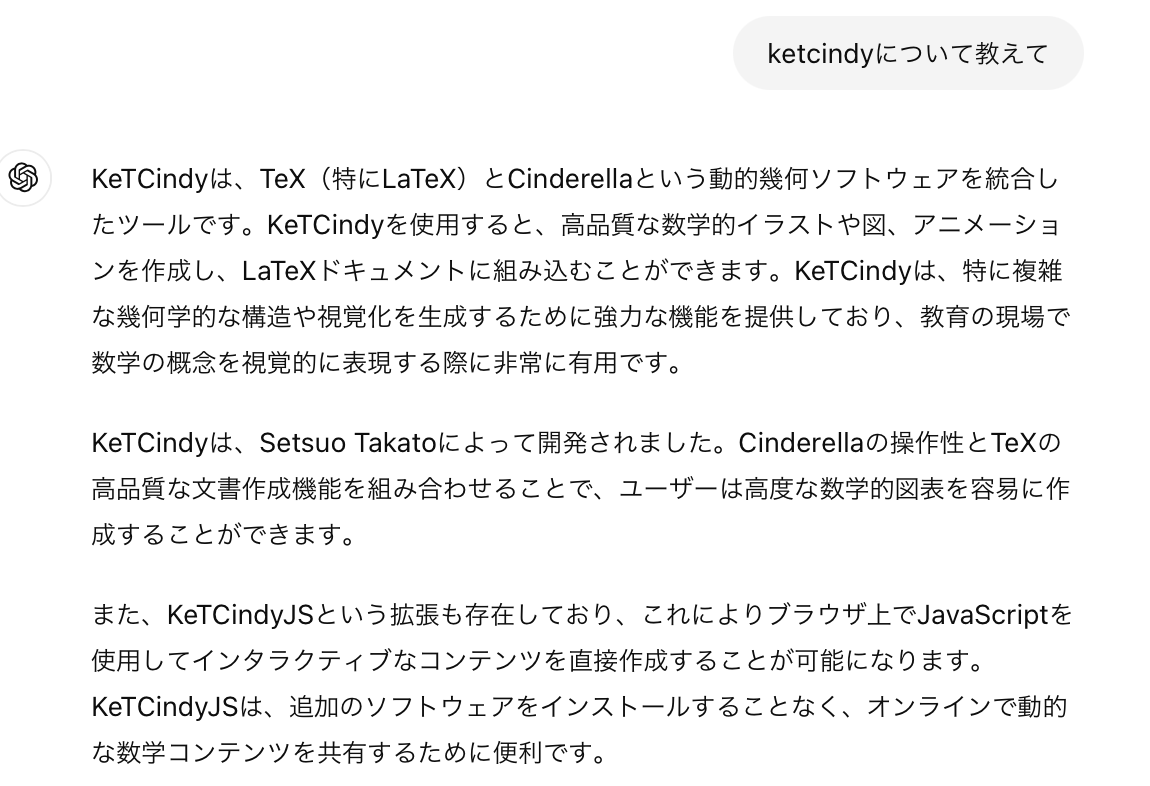
\includegraphics[width=100mm]{fig/chatgptketcindy.png}
\end{center}

\mainslide{KeTLMS}


\slidepage[m]
%%%%%%%%%%%%%

%%%%%%%%%%%%%%%%%%%%

\newslide{KeTLMSの開発}

\vspace*{18mm}

\slidepage
\textinit

\begin{layer}{120}{0}
\end{layer}

%%%%%%%%%%%%%

%%%%%%%%%%%%%%%%%%%%


\sameslide

\vspace*{18mm}

\slidepage
\textinit

\begin{layer}{120}{0}
\addtext{12}{\ten}{コロナ禍で開発を開始(2020)}
\end{layer}


\sameslide

\vspace*{18mm}

\slidepage
\textinit

\begin{layer}{120}{0}
\addtext{12}{\ten}{コロナ禍で開発を開始(2020)}
\addtext{12}{\ten}{教員と学生が課題の送受をするためのもの}
\end{layer}


\sameslide

\vspace*{18mm}

\slidepage
\textinit

\begin{layer}{120}{0}
\addtext{12}{\ten}{コロナ禍で開発を開始(2020)}
\addtext{12}{\ten}{教員と学生が課題の送受をするためのもの}
\addtext{12}{\ten}{数式の送受が難しい}
\end{layer}


\sameslide

\vspace*{18mm}

\slidepage
\textinit

\begin{layer}{120}{0}
\addtext{12}{\ten}{コロナ禍で開発を開始(2020)}
\addtext{12}{\ten}{教員と学生が課題の送受をするためのもの}
\addtext{12}{\ten}{数式の送受が難しい}
\addtext{20}{・}{簡易数式ルール(KeTMathルール)を設定}
\addtext{30}{}{\small str="fr(sin(x),cos(x))"}
\addtext[-3]{30}{}{\small Totexform(str)=\bs{dfrac{\bs{sin}x}{\bs{cos}x}}}
\addtext[-3]{30}{}{\small Tocindyform(str)="((sin(x))/(cos(x)))"}
\addtext[-3]{30}{}{\small Tomaxform(str)="((sin(x))/(cos(x)))"}
\end{layer}


\sameslide

\vspace*{18mm}

\slidepage
\textinit

\begin{layer}{120}{0}
\addtext{12}{\ten}{コロナ禍で開発を開始(2020)}
\addtext{12}{\ten}{教員と学生が課題の送受をするためのもの}
\addtext{12}{\ten}{数式の送受が難しい}
\addtext{20}{・}{簡易数式ルール(KeTMathルール)を設定}
\addtext{30}{}{\small str="fr(sin(x),cos(x))"}
\addtext[-3]{30}{}{\small Totexform(str)=\bs{dfrac{\bs{sin}x}{\bs{cos}x}}}
\addtext[-3]{30}{}{\small Tocindyform(str)="((sin(x))/(cos(x)))"}
\addtext[-3]{30}{}{\small Tomaxform(str)="((sin(x))/(cos(x)))"}
\addtext{12}{\ten}{\ketcindy JSを利用して雛形HTMLを作成}
\end{layer}


\newslide{コロナ後のKeTLMSの利用}

\vspace*{18mm}

\slidepage
\textinit

\begin{layer}{120}{0}
\addtext{8}{\ten}{通常の授業形態で利用}
\addtext{16}{・}{自習システムでない}
\end{layer}

%%%%%%%%%%%%%

%%%%%%%%%%%%%%%%%%%%


\sameslide

\vspace*{18mm}

\slidepage
\textinit

\begin{layer}{120}{0}
\addtext{8}{\ten}{通常の授業形態で利用}
\addtext{16}{・}{自習システムでない}
\addtext{8}{\ten}{オンラインでも対面でもよい}
\end{layer}


\sameslide

\vspace*{18mm}

\slidepage
\textinit

\begin{layer}{120}{0}
\addtext{8}{\ten}{通常の授業形態で利用}
\addtext{16}{・}{自習システムでない}
\addtext{8}{\ten}{オンラインでも対面でもよい}
\addtext{8}{\ten}{授業の途中で適宜質問を配付(ブレンド型授業)}
\end{layer}


\sameslide

\vspace*{18mm}

\slidepage
\textinit

\begin{layer}{120}{0}
\addtext{8}{\ten}{通常の授業形態で利用}
\addtext{16}{・}{自習システムでない}
\addtext{8}{\ten}{オンラインでも対面でもよい}
\addtext{8}{\ten}{授業の途中で適宜質問を配付(ブレンド型授業)}
\addtext{16}{・}{学生の進捗状況や理解度を見る}
\end{layer}


\sameslide

\vspace*{18mm}

\slidepage
\textinit

\begin{layer}{120}{0}
\addtext{8}{\ten}{通常の授業形態で利用}
\addtext{16}{・}{自習システムでない}
\addtext{8}{\ten}{オンラインでも対面でもよい}
\addtext{8}{\ten}{授業の途中で適宜質問を配付(ブレンド型授業)}
\addtext{16}{・}{学生の進捗状況や理解度を見る}
\addtext{16}{・}{報告者の場合,200分授業で5−8回}
\end{layer}


\sameslide

\vspace*{18mm}

\slidepage
\textinit

\begin{layer}{120}{0}
\addtext{8}{\ten}{通常の授業形態で利用}
\addtext{16}{・}{自習システムでない}
\addtext{8}{\ten}{オンラインでも対面でもよい}
\addtext{8}{\ten}{授業の途中で適宜質問を配付(ブレンド型授業)}
\addtext{16}{・}{学生の進捗状況や理解度を見る}
\addtext{16}{・}{報告者の場合,200分授業で5−8回}
\addtext{8}{\ten}{多様な出題形式に対応}
\end{layer}


\sameslide

\vspace*{18mm}

\slidepage
\textinit

\begin{layer}{120}{0}
\addtext{8}{\ten}{通常の授業形態で利用}
\addtext{16}{・}{自習システムでない}
\addtext{8}{\ten}{オンラインでも対面でもよい}
\addtext{8}{\ten}{授業の途中で適宜質問を配付(ブレンド型授業)}
\addtext{16}{・}{学生の進捗状況や理解度を見る}
\addtext{16}{・}{報告者の場合,200分授業で5−8回}
\addtext{8}{\ten}{多様な出題形式に対応}
\addtext{8}{\ten}{成績処理は授業後}
\end{layer}


\newslide{kettask.htmlの作成(準備)}

\vspace*{18mm}

\slidepage
\textinit

\begin{layer}{120}{0}
\addtext{8}{\ten}{`ketcindy home'で検索,KeT-LMSのファイル1式(ketmath)をDL,Unzip}
\end{layer}

%%%%%%%%%%%%%

%%%%%%%%%%%%%%%%%%%%


\sameslide

\vspace*{18mm}

\slidepage
\textinit

\begin{layer}{120}{0}
\addtext{8}{\ten}{`ketcindy home'で検索,KeT-LMSのファイル1式(ketmath)をDL,Unzip}
\addtext[8]{8}{\ten}{subject01を用いる}
\addtext{16}{・}{\ketcindy のライブラリも同梱しているので,Cinderellaだけあれば,そのまま使える}
\end{layer}


\sameslide

\vspace*{18mm}

\slidepage
\textinit

\begin{layer}{120}{0}
\addtext{8}{\ten}{`ketcindy home'で検索,KeT-LMSのファイル1式(ketmath)をDL,Unzip}
\addtext[8]{8}{\ten}{subject01を用いる}
\addtext{16}{・}{\ketcindy のライブラリも同梱しているので,Cinderellaだけあれば,そのまま使える}
\addtext[8]{8}{\ten}{dataにあるstudent.txtに学生リストを書く}
\addtext{20}{}{\small 01AA}
\addtext[-3]{20}{}{\small 02BB}
\addtext[-3]{20}{}{\small ...}
\end{layer}


\newslide{問題ファイルの作成}

\vspace*{18mm}

\slidepage
\textinit

\begin{layer}{120}{0}
\addtext{8}{\ten}{question(id).txtをdataに作成}
\addtext{16}{}{\small y = a$\;\hat{}\;$(x)について,a$>$0, a(neq)1とする}
\addtext[-3]{16}{}{\small [1] aの値を入力してOKを押せ}
\addtext[-3]{16}{}{\small [2] グラフとy軸との交点を入力してOKを押せ}
\addtext[-3]{16}{}{\small Sheet}
\addtext[-3]{16}{}{\small [1] a=? :{}:2:{}:-1}
\addtext[-3]{16}{}{\small [2] (0,?) :{}:2}
\addtext[-3]{16}{}{\small Ans}
\addtext[-3]{16}{}{\small [1]}
\addtext[-3]{16}{}{\small [2]}
\end{layer}

%%%%%%%%%%%%%

%%%%%%%%%%%%%%%%%%%%


\newslide{kettask.htmlの作成}

\vspace*{18mm}

\slidepage
\vspace{-2mm}

\textinit

\begin{layer}{120}{0}
\addtext{8}{\ten}{toolketmath.cdyを立ち上げる}
\putnotes{68}{15}{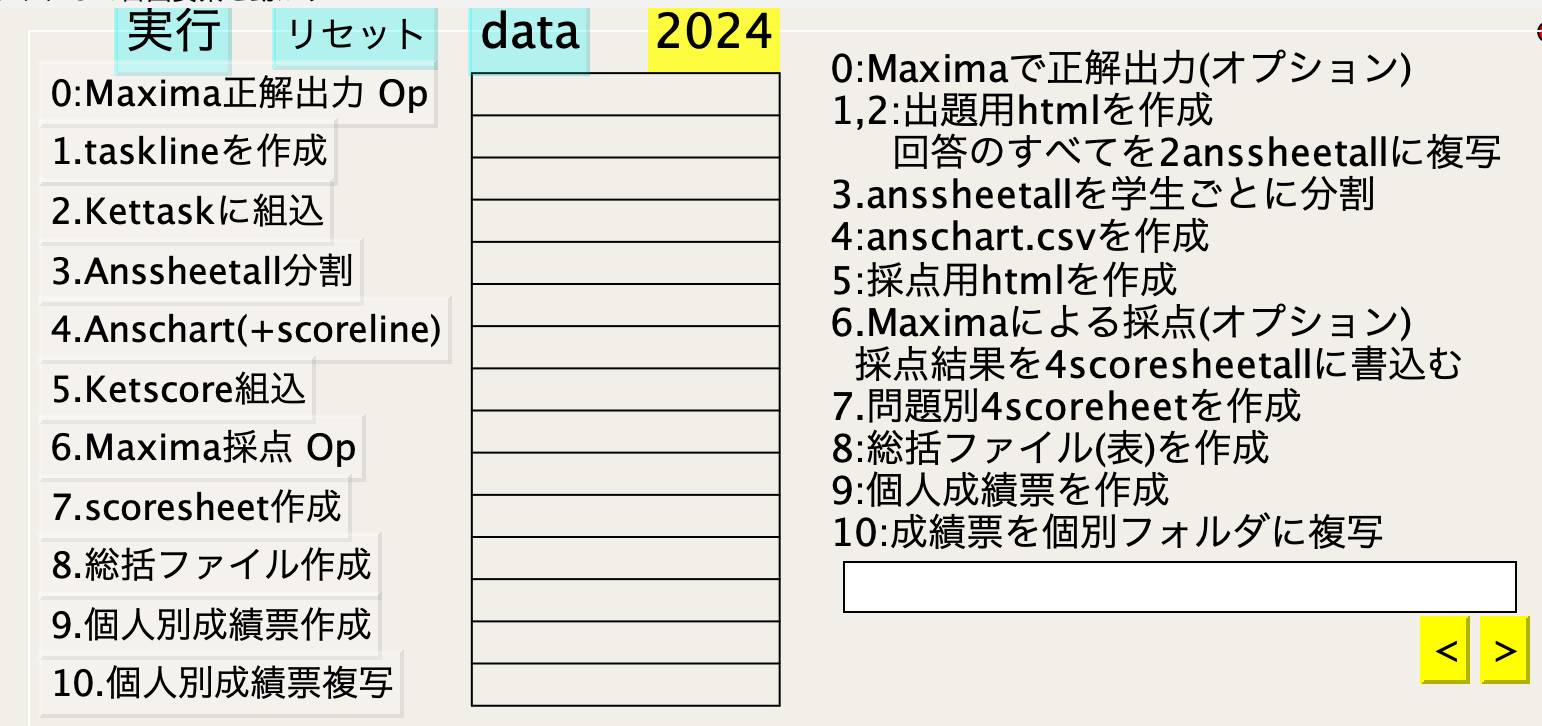
\includegraphics[height=46mm]{fig/toolketmath.png}}
\end{layer}

%%%%%%%%%%%%%

%%%%%%%%%%%%%%%%%%%%


\sameslide

\vspace*{18mm}

\slidepage
\vspace{-2mm}

\textinit

\begin{layer}{120}{0}
\addtext{8}{\ten}{toolketmath.cdyを立ち上げる}
\putnotes{68}{15}{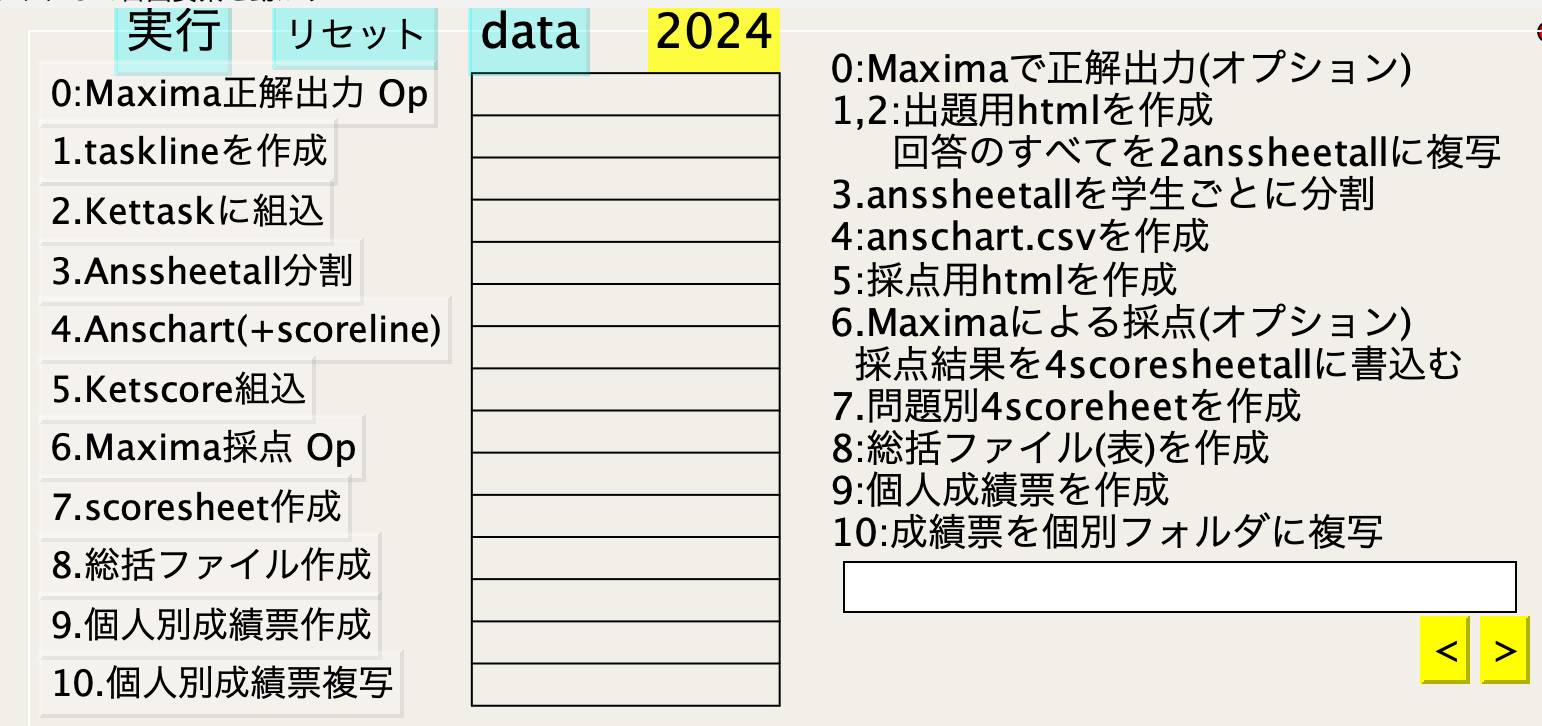
\includegraphics[height=46mm]{fig/toolketmath.png}}
\addtext[48]{8}{\ten}{1.taskline を実行}
\end{layer}


\sameslide

\vspace*{18mm}

\slidepage
\vspace{-2mm}

\textinit

\begin{layer}{120}{0}
\addtext{8}{\ten}{toolketmath.cdyを立ち上げる}
\putnotes{68}{15}{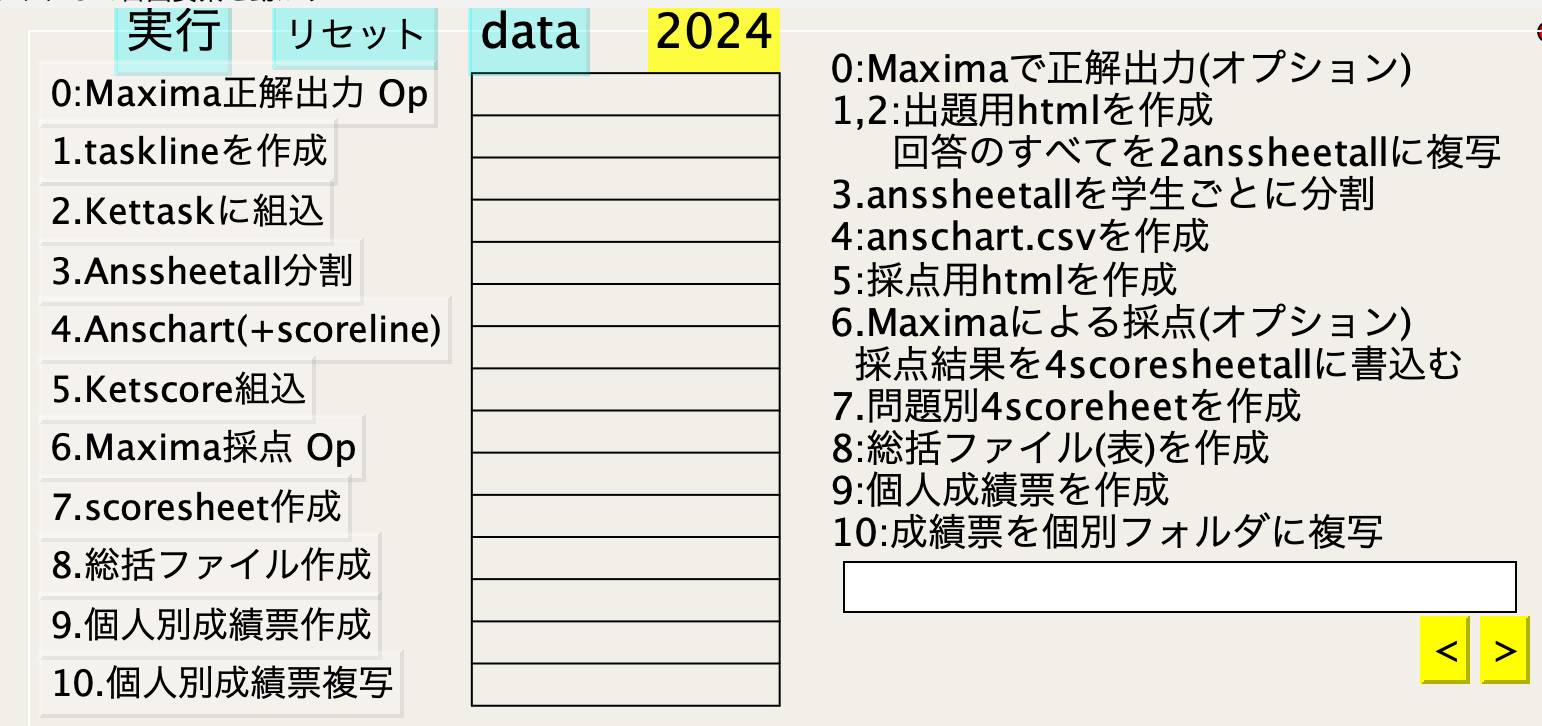
\includegraphics[height=46mm]{fig/toolketmath.png}}
\addtext[48]{8}{\ten}{1.taskline を実行}
\addtext{8}{\ten}{3.Kettaskに組込 を実行}
\end{layer}


\sameslide

\vspace*{18mm}

\slidepage
\textinit

\begin{layer}{120}{0}
\putnotes{68}{0}{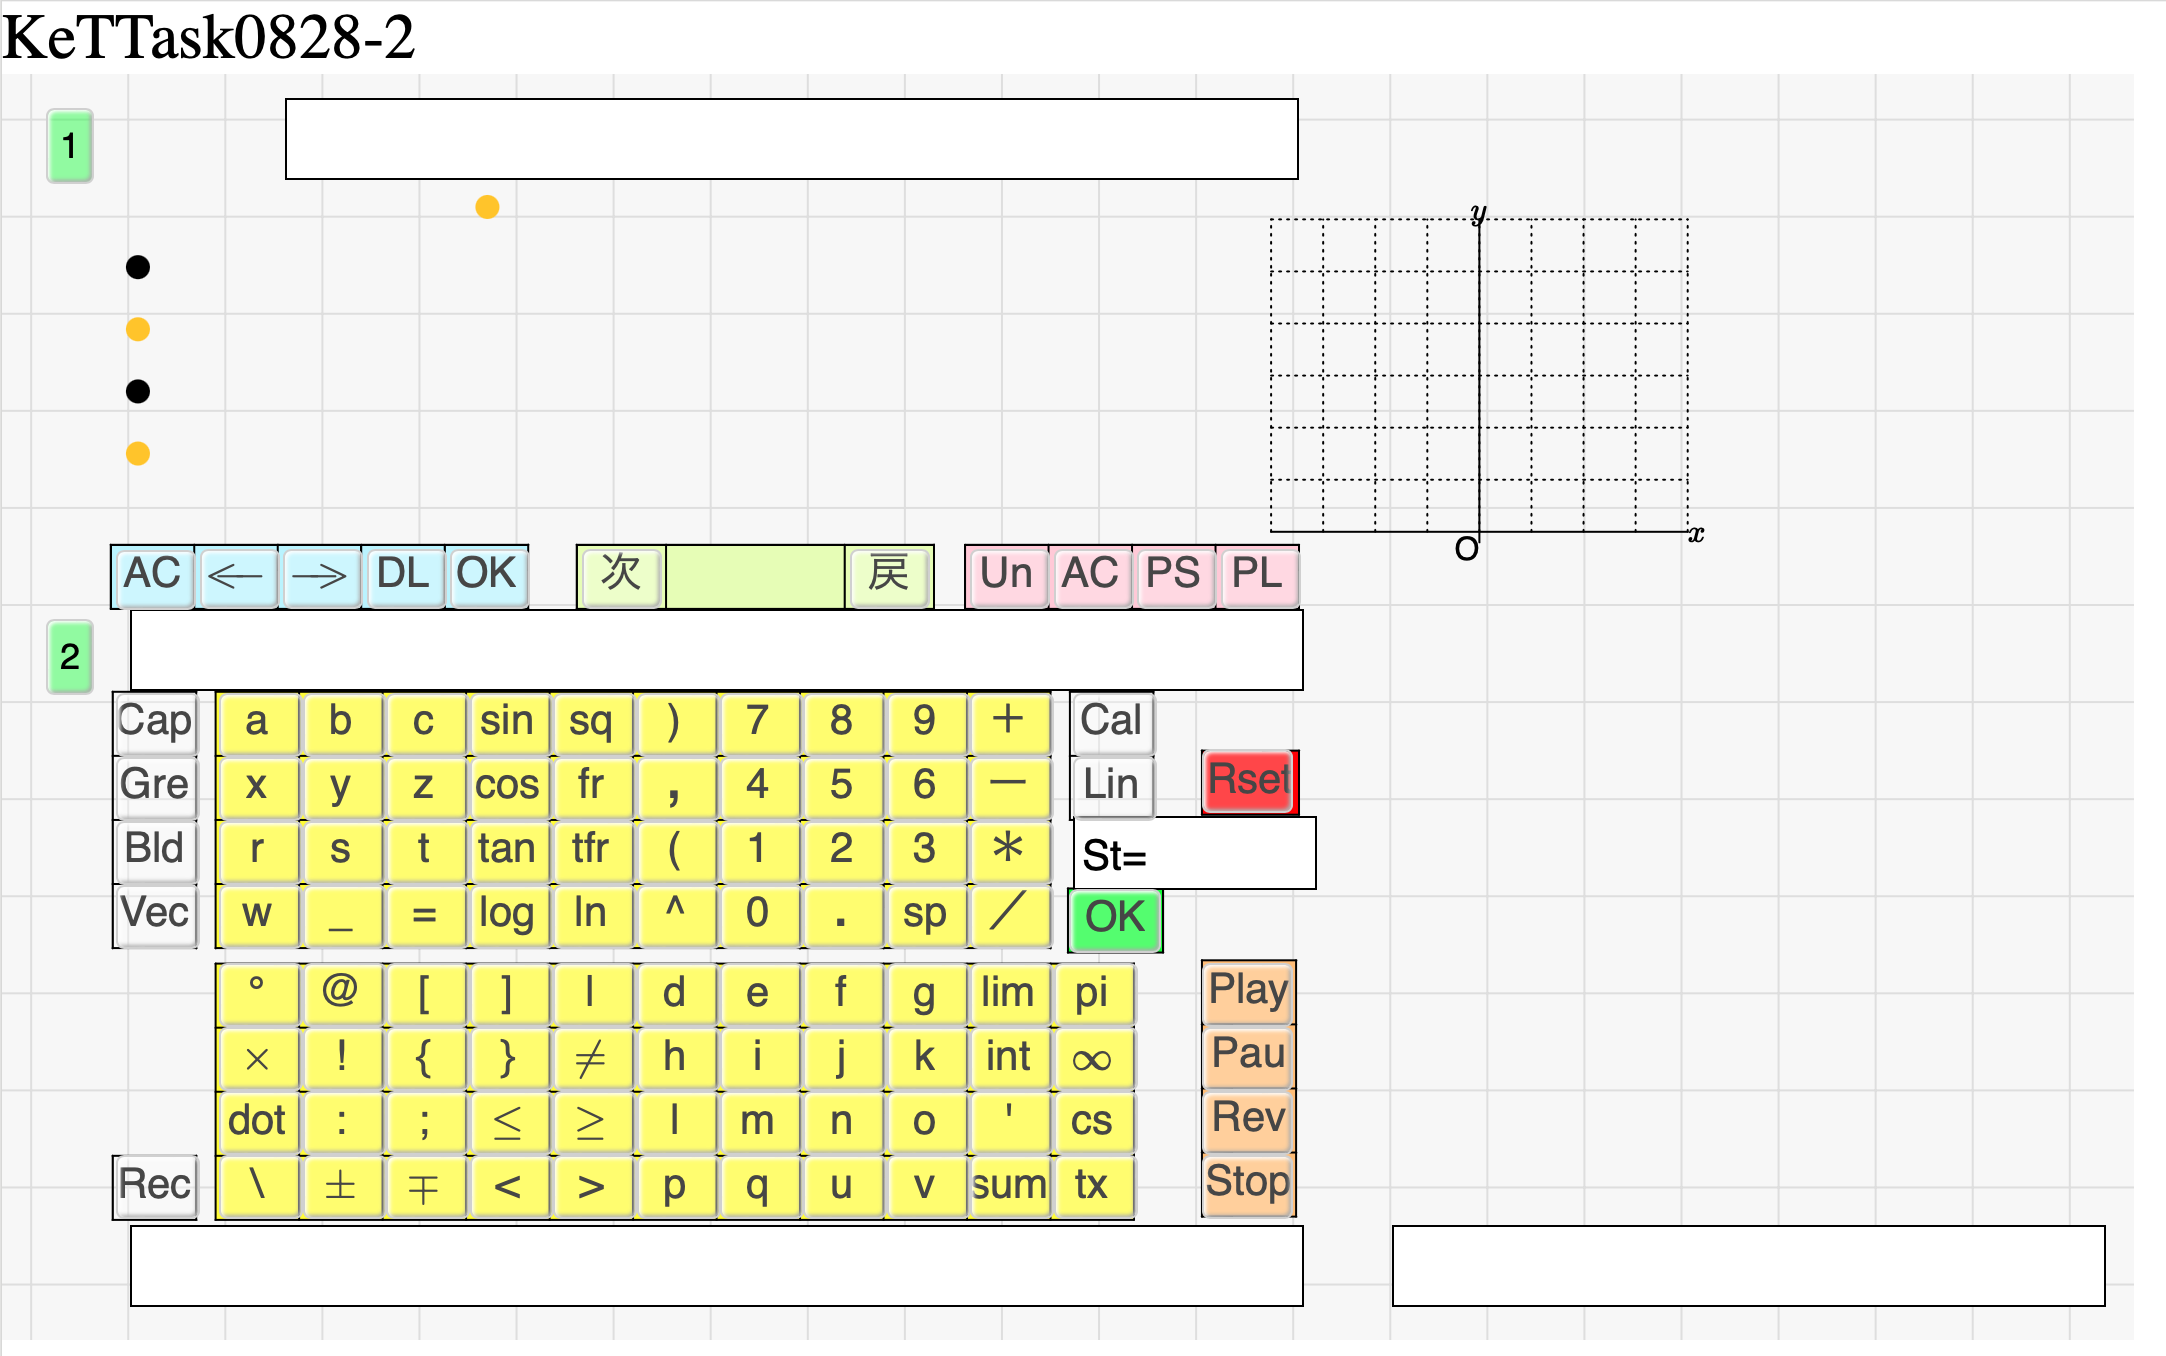
\includegraphics[height=70mm]{fig/kettask.png}}
\end{layer}

%%%%%%%%%%%%%

%%%%%%%%%%%%%%%%%%%%


\newslide{KeTLMSの実際(デモ)}

\vspace*{18mm}

\slidepage
\textinit

\begin{layer}{120}{0}
\addtext{8}{\ten}{沼津高専の学生さんに手伝ってもらいます}
\end{layer}

%%%%%%%%%%%%%

%%%%%%%%%%%%%%%%%%%%


\sameslide

\vspace*{18mm}

\slidepage
\textinit

\begin{layer}{120}{0}
\addtext{8}{\ten}{沼津高専の学生さんに手伝ってもらいます}
\addtext{8}{\ten}{kettask.htmlをGitHub/Pagesにアップ}
\end{layer}


\sameslide

\vspace*{18mm}

\slidepage
\textinit

\begin{layer}{120}{0}
\addtext{8}{\ten}{沼津高専の学生さんに手伝ってもらいます}
\addtext{8}{\ten}{kettask.htmlをGitHub/Pagesにアップ}
\addtext{8}{\ten}{GoogleClassroom(GC)でURLを配付}
\end{layer}


\sameslide

\vspace*{18mm}

\slidepage
\textinit

\begin{layer}{120}{0}
\addtext{8}{\ten}{沼津高専の学生さんに手伝ってもらいます}
\addtext{8}{\ten}{kettask.htmlをGitHub/Pagesにアップ}
\addtext{8}{\ten}{GoogleClassroom(GC)でURLを配付}
\addtext{8}{\ten}{学生は回答を作り,GCで提出}
\end{layer}


\sameslide

\vspace*{18mm}

\slidepage
\textinit

\begin{layer}{120}{0}
\addtext{8}{\ten}{沼津高専の学生さんに手伝ってもらいます}
\addtext{8}{\ten}{kettask.htmlをGitHub/Pagesにアップ}
\addtext{8}{\ten}{GoogleClassroom(GC)でURLを配付}
\addtext{8}{\ten}{学生は回答を作り,GCで提出}
\addtext{8}{\ten}{集積した回答により成績処理}
\end{layer}


\newslide{まとめ}

\vspace*{18mm}

\slidepage
\vspace{-2mm}

\textinit

\begin{layer}{120}{0}
\addtext{8}{\ten}{?による入力位置の指定}
\addtext{16}{}{学生のミスが激減}
\addtext{16}{}{多様な出題形式}
\end{layer}

%%%%%%%%%%%%%

%%%%%%%%%%%%%%%%%%%%


\sameslide

\vspace*{18mm}

\slidepage
\vspace{-2mm}

\textinit

\begin{layer}{120}{0}
\addtext{8}{\ten}{?による入力位置の指定}
\addtext{16}{}{学生のミスが激減}
\addtext{16}{}{多様な出題形式}
\addtext{8}{\ten}{中間試験ですべての学生がKeTLMSを希望}
\putnotes{68}{39}{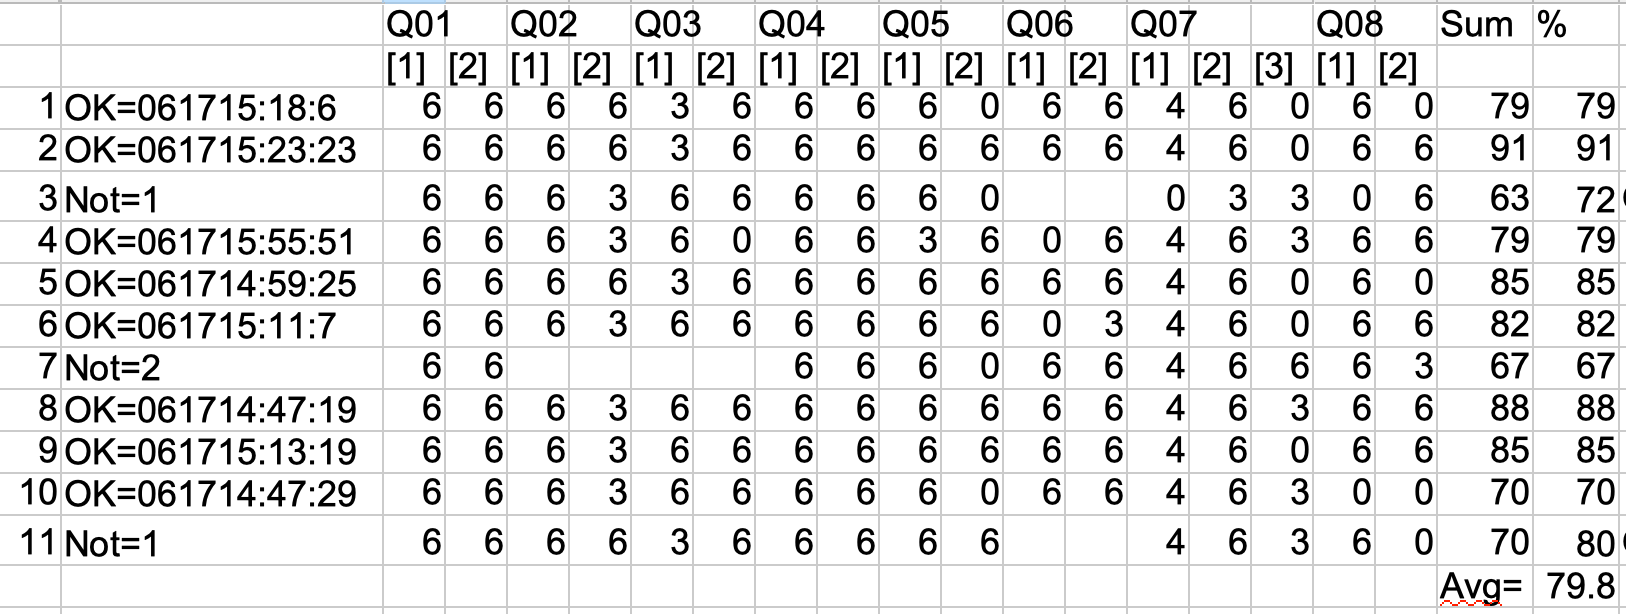
\includegraphics[height=40mm]{fig/2024-1res.png}}
\end{layer}


\sameslide

\vspace*{18mm}

\slidepage
\textinit

\begin{layer}{120}{0}
\addtext{8}{\ten}{学生は喜んで取り組んでいる}
\end{layer}


\sameslide

\vspace*{18mm}

\slidepage
\textinit

\begin{layer}{120}{0}
\addtext{8}{\ten}{学生は喜んで取り組んでいる}
\addtext{8}{\ten}{1期9回で73問}
\end{layer}


\sameslide

\vspace*{18mm}

\slidepage
\textinit

\begin{layer}{120}{0}
\addtext{8}{\ten}{学生は喜んで取り組んでいる}
\addtext{8}{\ten}{1期9回で73問}
\addtext{8}{\ten}{ペーパーレス}
\addtext{16}{}{配付プリントは事務作成のシラバス}
\end{layer}


\sameslide

\vspace*{18mm}

\slidepage
\textinit

\begin{layer}{120}{0}
\addtext{8}{\ten}{学生は喜んで取り組んでいる}
\addtext{8}{\ten}{1期9回で73問}
\addtext{8}{\ten}{ペーパーレス}
\addtext{16}{}{配付プリントは事務作成のシラバス}
\addtext{8}{\ten}{データはすべてテキストファイル}
\addtext{16}{・}{加工が容易}
\addtext{16}{・}{長期間有効}
\addtext{24}{}{\TeX\ 1976,Word 1983,Appleworks 1993}
\end{layer}


\sameslide

\vspace*{18mm}

\slidepage
\textinit

\begin{layer}{120}{0}
\addtext{8}{\ten}{学生は喜んで取り組んでいる}
\addtext{8}{\ten}{1期9回で73問}
\addtext{8}{\ten}{ペーパーレス}
\addtext{16}{}{配付プリントは事務作成のシラバス}
\addtext{8}{\ten}{データはすべてテキストファイル}
\addtext{16}{・}{加工が容易}
\addtext{16}{・}{長期間有効}
\addtext{24}{}{\TeX\ 1976,Word 1983,Appleworks 1993}
\end{layer}

\label{pageend}\mbox{}

\end{document}
